\chapter{Réalisation et tests}

% ─────────────────────────────────────────────────────────────────────────────
\section{Introduction}

Ce chapitre présente la phase de réalisation du système et les résultats obtenus.
La préparation des données et la mise en place des modèles d'IA ayant été traitées
au Chapitre~5, ce chapitre couvre l'environnement de développement,
les interfaces réalisées, les tests effectués,
les aspects de sécurité selon le référentiel OWASP Top~10 for LLM Applications,
l'évaluation de la qualité des réponses avec le framework RAGAS,
les optimisations de performance et le déploiement.

% ─────────────────────────────────────────────────────────────────────────────
\section{Environnement de développement}

\subsection{Environnement matériel et logiciel}

Le développement a été réalisé sur des machines sous Windows~11 avec accès au serveur
d'inférence kaisens.fr.
Le Tableau~\ref{tab:env_dev} présente les outils et technologies utilisés.

\vspace{6pt}
\begin{table}[H]
\centering
\caption{Environnement de développement}
\label{tab:env_dev}
\begin{tabular}{|l|l|}
\hline
\textbf{Catégorie} & \textbf{Outil / Version} \\
\hline
Langage principal & Python 3.11 \\
Langage traitement de données & Scala 2.12.18 / Apache Spark 3.5 \\
Interface interne & Streamlit 1.32 \\
Interface publique & React 18 + Vite \\
Backend API & FastAPI 0.110 \\
Orchestration LLM & LangChain 0.2 \\
Base documentaire & ChromaDB 0.5 \\
Mémoire de session & Redis 7.2 \\
Évaluation RAG & RAGAS 0.1 (juge LLM : Groq API) \\
Conteneurisation & Docker / Docker Compose \\
Contrôle de version & Git / GitLab (\texttt{gitlab.dataforethic.fr}) \\
\hline
\end{tabular}
\end{table}

% ─────────────────────────────────────────────────────────────────────────────
\section{Module 1 — Noa : assistant virtuel du site public}

\subsection{Tests}

Une suite de 46~tests automatisés couvre l'ensemble des fonctionnalités de Noa.
Le Tableau~\ref{tab:tests_noa} présente les résultats obtenus.

\vspace{6pt}
\begin{table}[H]
\centering
\caption{Résultats des tests automatisés — Module Noa}
\label{tab:tests_noa}
\begin{tabular}{|l|c|c|}
\hline
\textbf{Catégorie de test} & \textbf{Nombre} & \textbf{Résultat} \\
\hline
Routage par intention & 8 & 100\,\% \\
Recherche documentaire & 10 & 100\,\% \\
Agent de réservation & 12 & 100\,\% \\
Mémoire et cache & 8 & 100\,\% \\
Gestion des erreurs & 8 & 100\,\% \\
\hline
\textbf{Total} & \textbf{46} & \textbf{100\,\%} \\
\hline
\end{tabular}
\end{table}

\subsection{Performances}

Le Tableau~\ref{tab:perf_noa} présente les temps de réponse mesurés pour chaque type de requête.

\vspace{6pt}
\begin{table}[H]
\centering
\caption{Temps de réponse moyens — Module Noa}
\label{tab:perf_noa}
\begin{tabular}{|l|c|c|}
\hline
\textbf{Type de requête} & \textbf{Temps moyen} & \textbf{Exigence} \\
\hline
Réponse depuis le cache & $<$ 1\,ms & $<$ 50\,ms \\
Salutation / hors sujet & $<$ 10\,ms & $<$ 100\,ms \\
Question factuelle (RAG) & $\approx$ 1,8\,s & $<$ 5\,s \\
Question de suivi & $\approx$ 2,1\,s & $<$ 5\,s \\
\hline
\end{tabular}
\end{table}

% ─────────────────────────────────────────────────────────────────────────────
\section{Module 2 — NetEthic Support Assistant}

\subsection{Interface utilisateur}

La Figure~\ref{fig:support_interface} montre l'interface principale du Support Assistant.

\begin{figure}[H]
\centering
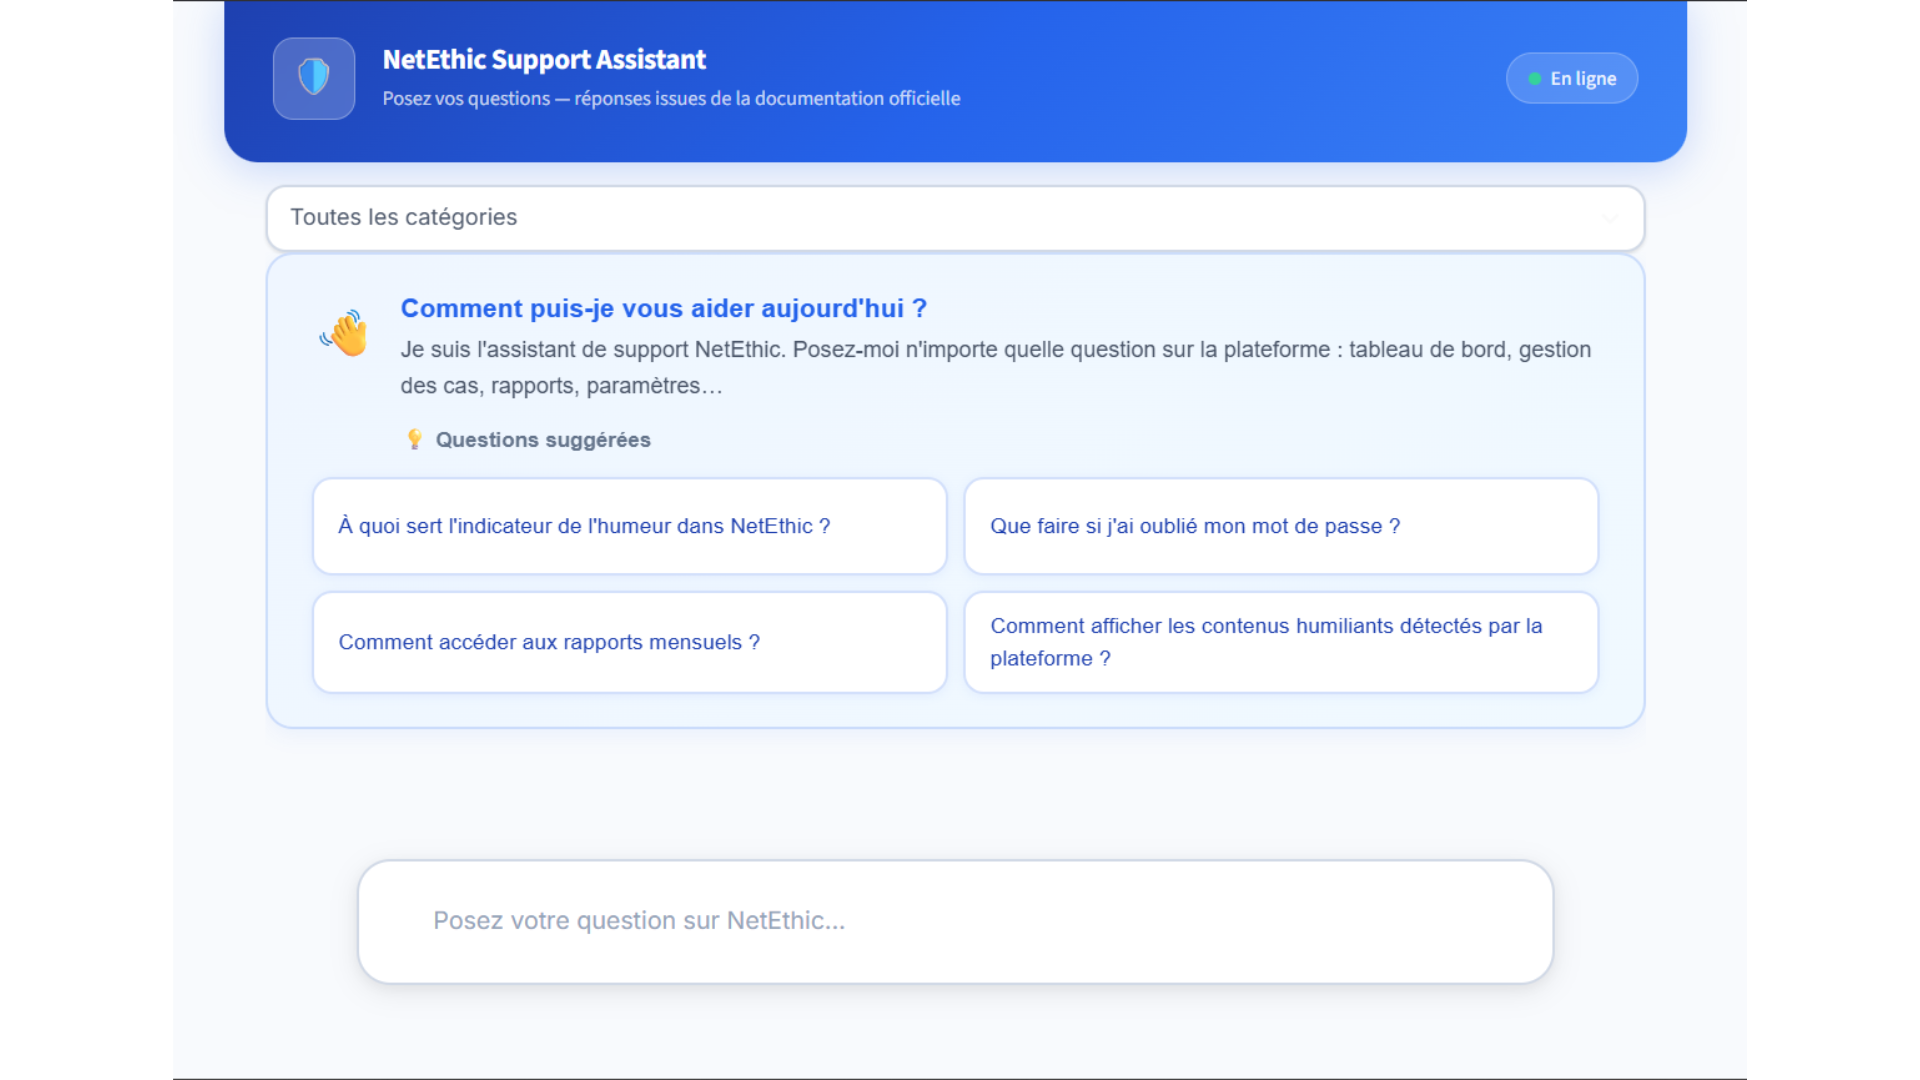
\includegraphics[width=0.85\textwidth]{interface-png/acceuil-support-chatbot.png}
\caption{Interface principale du NetEthic Support Assistant}
\label{fig:support_interface}
\end{figure}

\subsection{Interface contact support}

Lorsque le Support Assistant ne trouve pas de réponse dans la documentation,
il propose automatiquement trois actions à l'utilisateur : planifier un rendez-vous,
signaler un dysfonctionnement, ou accéder directement au portail de support en ligne.
La Figure~\ref{fig:support_contact} illustre cet écran d'actions.

\begin{figure}[H]
\centering
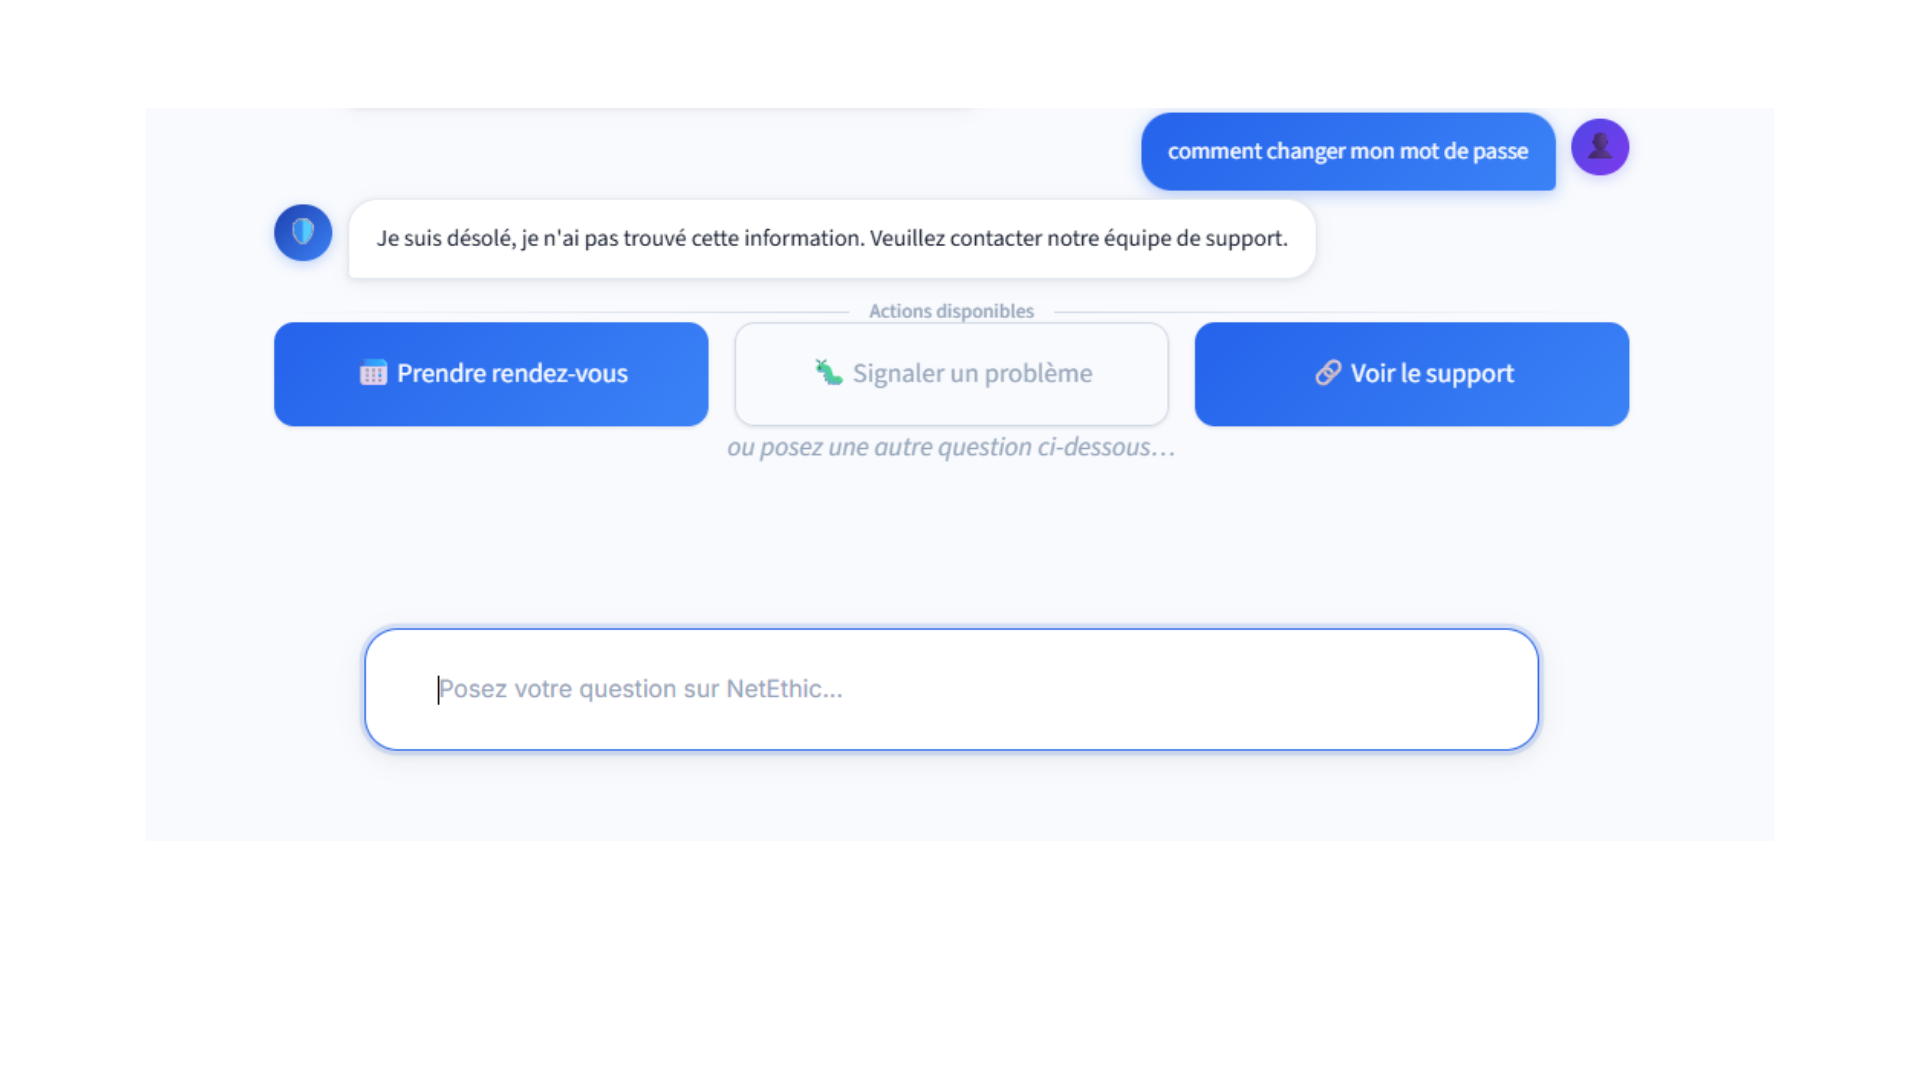
\includegraphics[width=0.85\textwidth]{interface-png/contact-support-interface.png}
\caption{Support Assistant — écran \og Contacter le support \fg{} avec les trois actions disponibles}
\label{fig:support_contact}
\end{figure}

\subsubsection{Flux de réservation de rendez-vous}

Lorsque l'utilisateur choisit \og Prendre rendez-vous \fg{}, un formulaire guidé en quatre étapes
s'ouvre directement dans la fenêtre de conversation.
Le motif du rendez-vous est pré-rempli automatiquement à partir du contexte de la conversation
(BF-S07), sans que l'utilisateur ait à ressaisir ses informations (BF-S09).
La Figure~\ref{fig:support_rdv_heure} montre l'étape de saisie de l'heure (étape~2/4),
et la Figure~\ref{fig:support_rdv_confirm} présente l'écran de confirmation finale (étape~4/4)
avec le résumé complet du rendez-vous avant envoi.

\begin{figure}[H]
\centering
\begin{subfigure}[t]{0.49\textwidth}
  \centering
  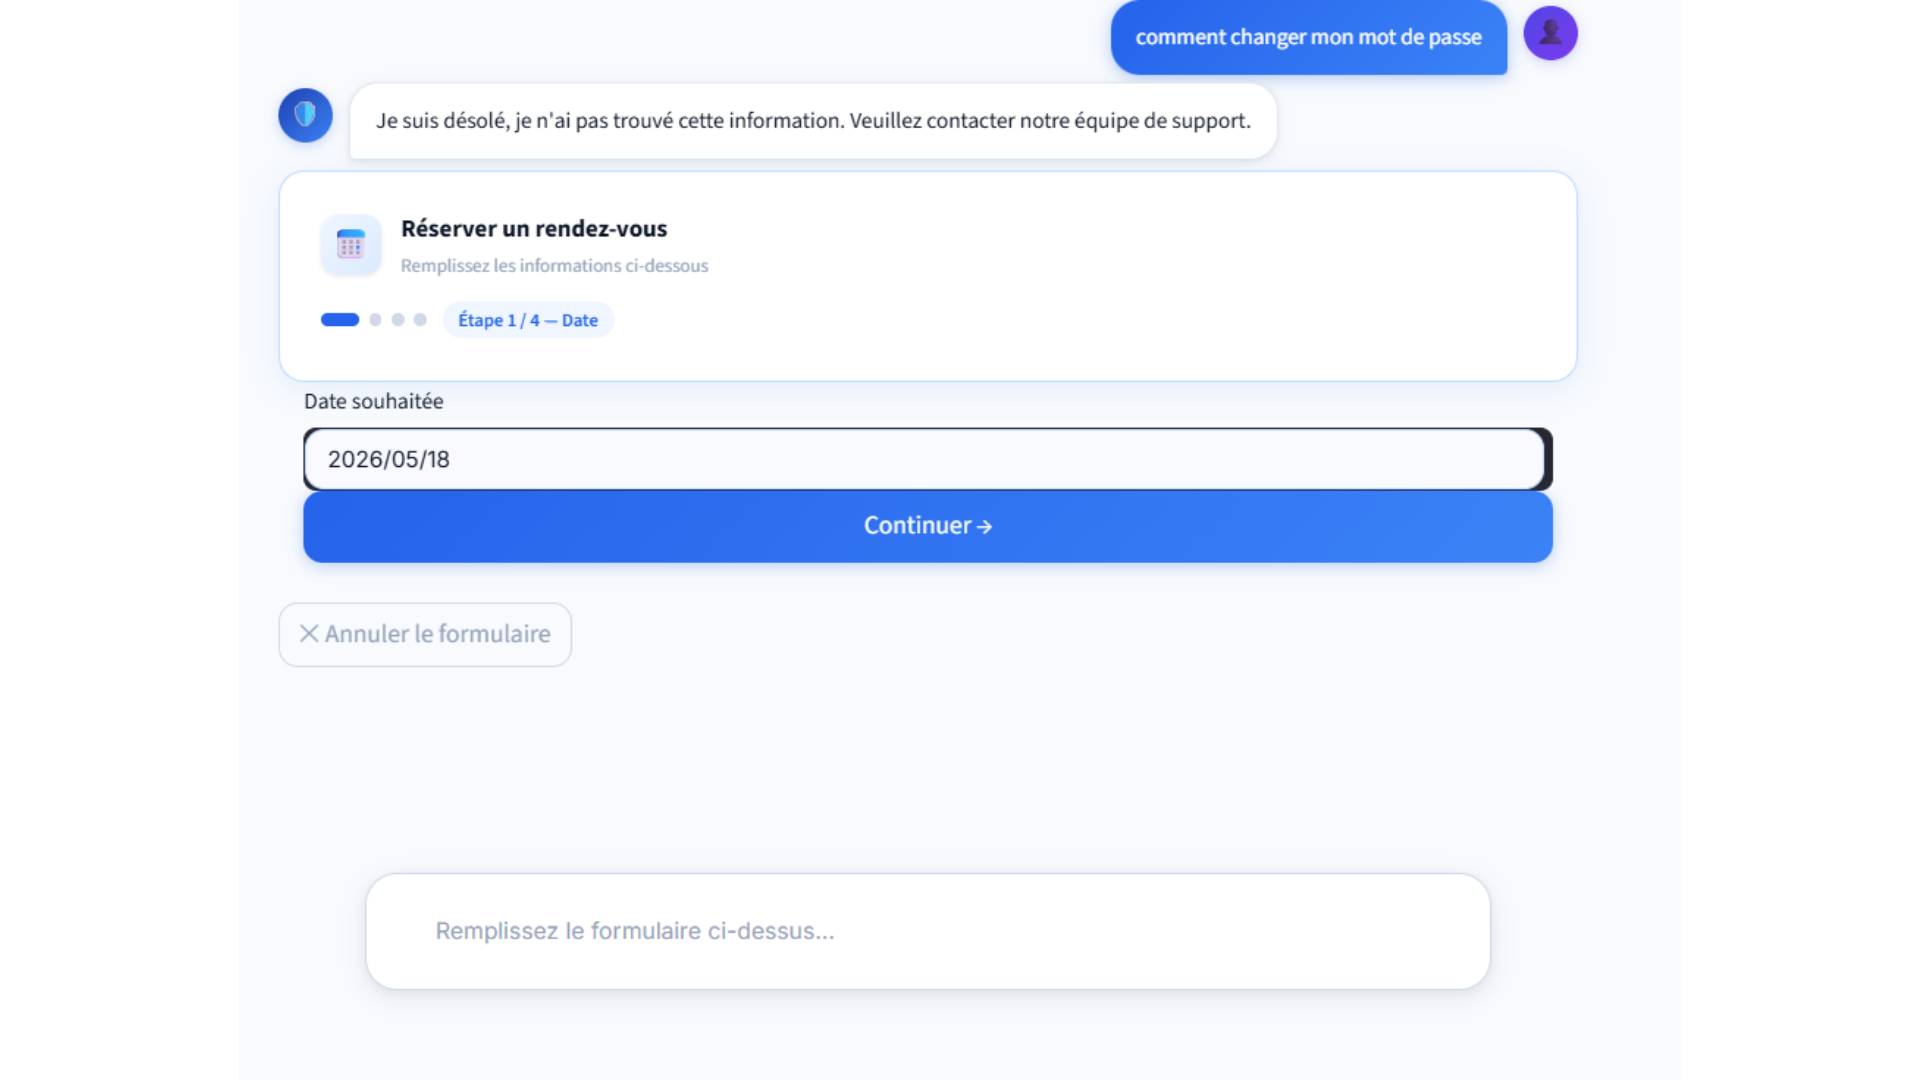
\includegraphics[width=\textwidth]{interface-png/rendez-vous-interface4.png}
  \caption{Étape 1/4 — date souhaitée}
  \label{fig:support_rdv_date}
\end{subfigure}
\hfill
\begin{subfigure}[t]{0.49\textwidth}
  \centering
  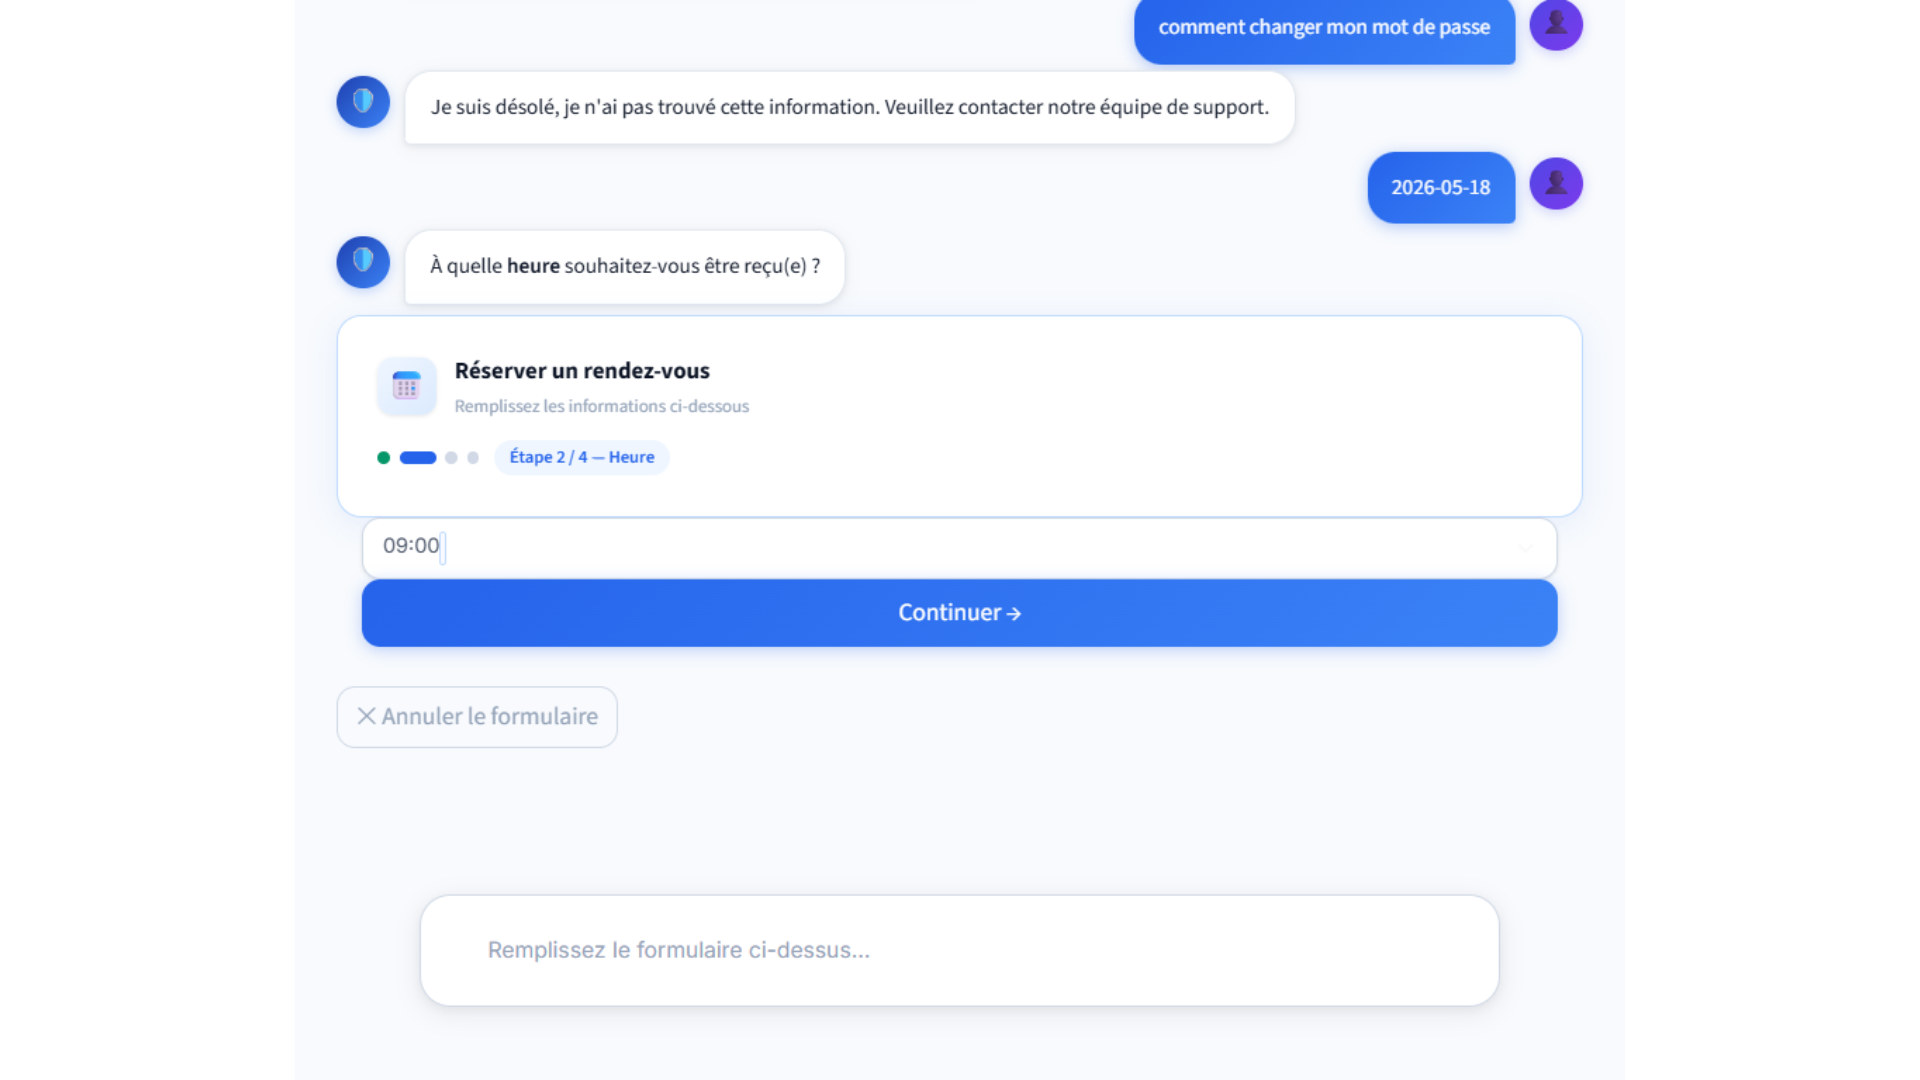
\includegraphics[width=\textwidth]{interface-png/rendez-vous-interface2.png}
  \caption{Étape 2/4 — heure souhaitée}
  \label{fig:support_rdv_heure}
\end{subfigure}

\vspace{8pt}

\begin{subfigure}[t]{0.49\textwidth}
  \centering
  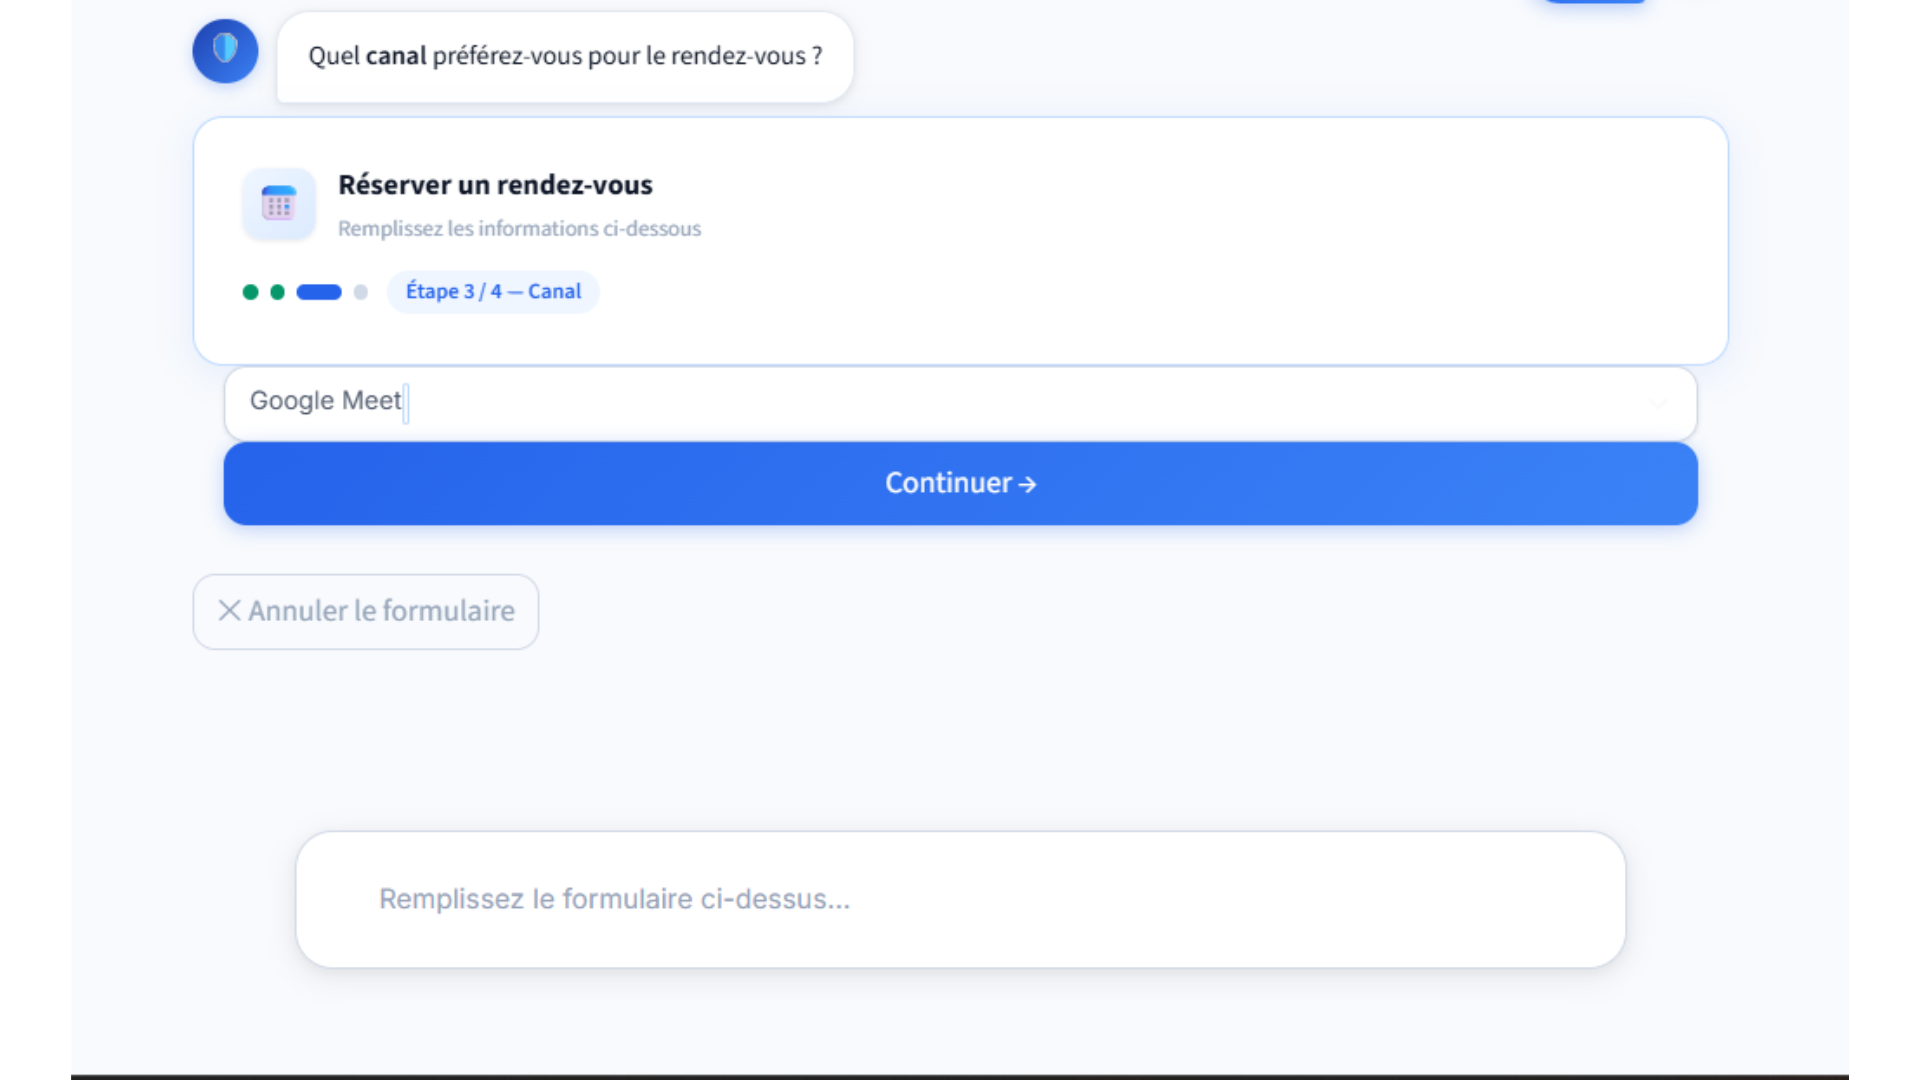
\includegraphics[width=\textwidth]{interface-png/rendez-vous-interface3.png}
  \caption{Étape 3/4 — canal préféré}
  \label{fig:support_rdv_canal}
\end{subfigure}
\hfill
\begin{subfigure}[t]{0.49\textwidth}
  \centering
  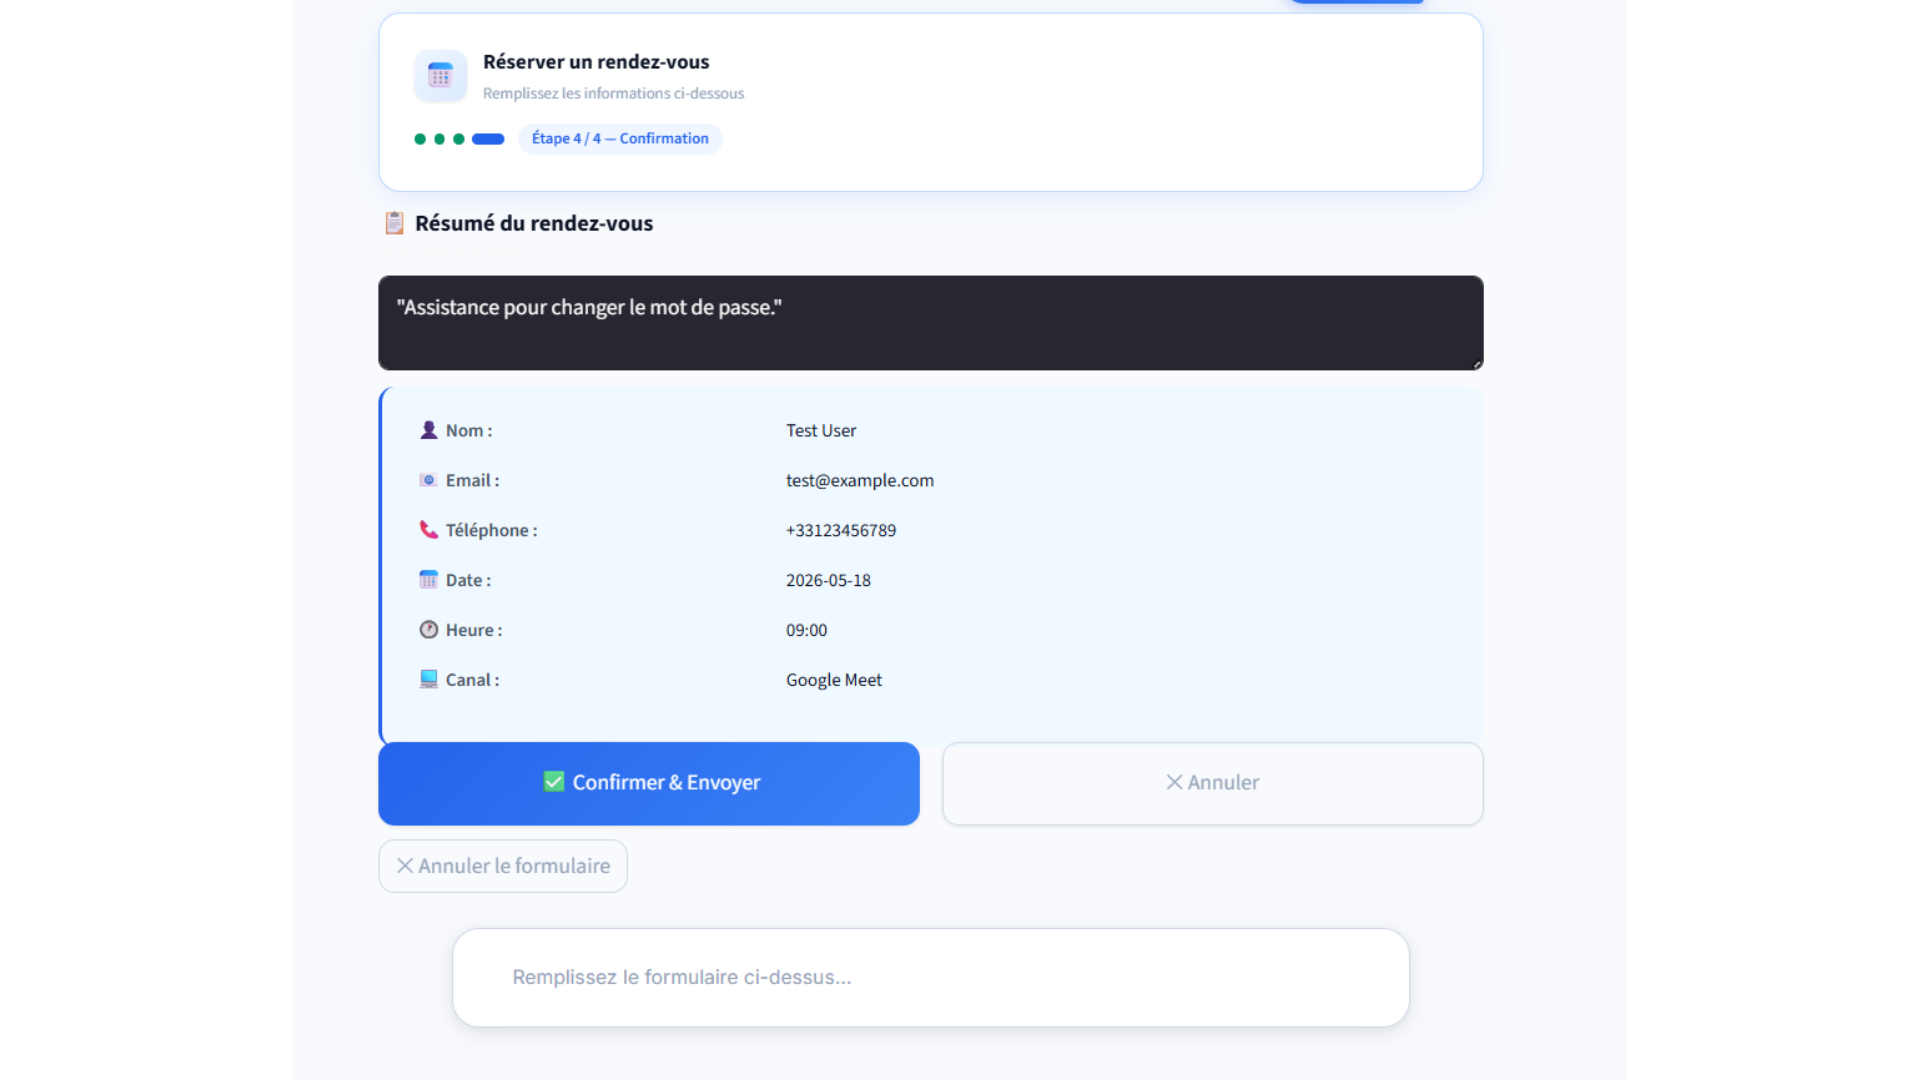
\includegraphics[width=\textwidth]{interface-png/rendez-vous-interface.png}
  \caption{Étape 4/4 — confirmation et résumé}
  \label{fig:support_rdv_confirm}
\end{subfigure}
\caption{Support Assistant — formulaire guidé de prise de rendez-vous (4 étapes)}
\label{fig:support_rdv}
\end{figure}

\subsubsection{Flux de signalement de dysfonctionnement}

Lorsque l'utilisateur choisit \og Signaler un problème \fg{}, un formulaire en trois étapes
s'affiche dans la conversation.
À l'étape~2, la description du problème est générée automatiquement par le LLM
à partir de l'historique de la conversation (BF-S07), puis reste modifiable avant envoi.
La Figure~\ref{fig:support_bug_desc} illustre cette étape avec la description auto-générée,
et la Figure~\ref{fig:support_bug_confirm} présente l'écran de confirmation finale (étape~3/3)
avant transmission à l'équipe technique.

\begin{figure}[H]
\centering
\begin{subfigure}[t]{0.48\textwidth}
  \centering
  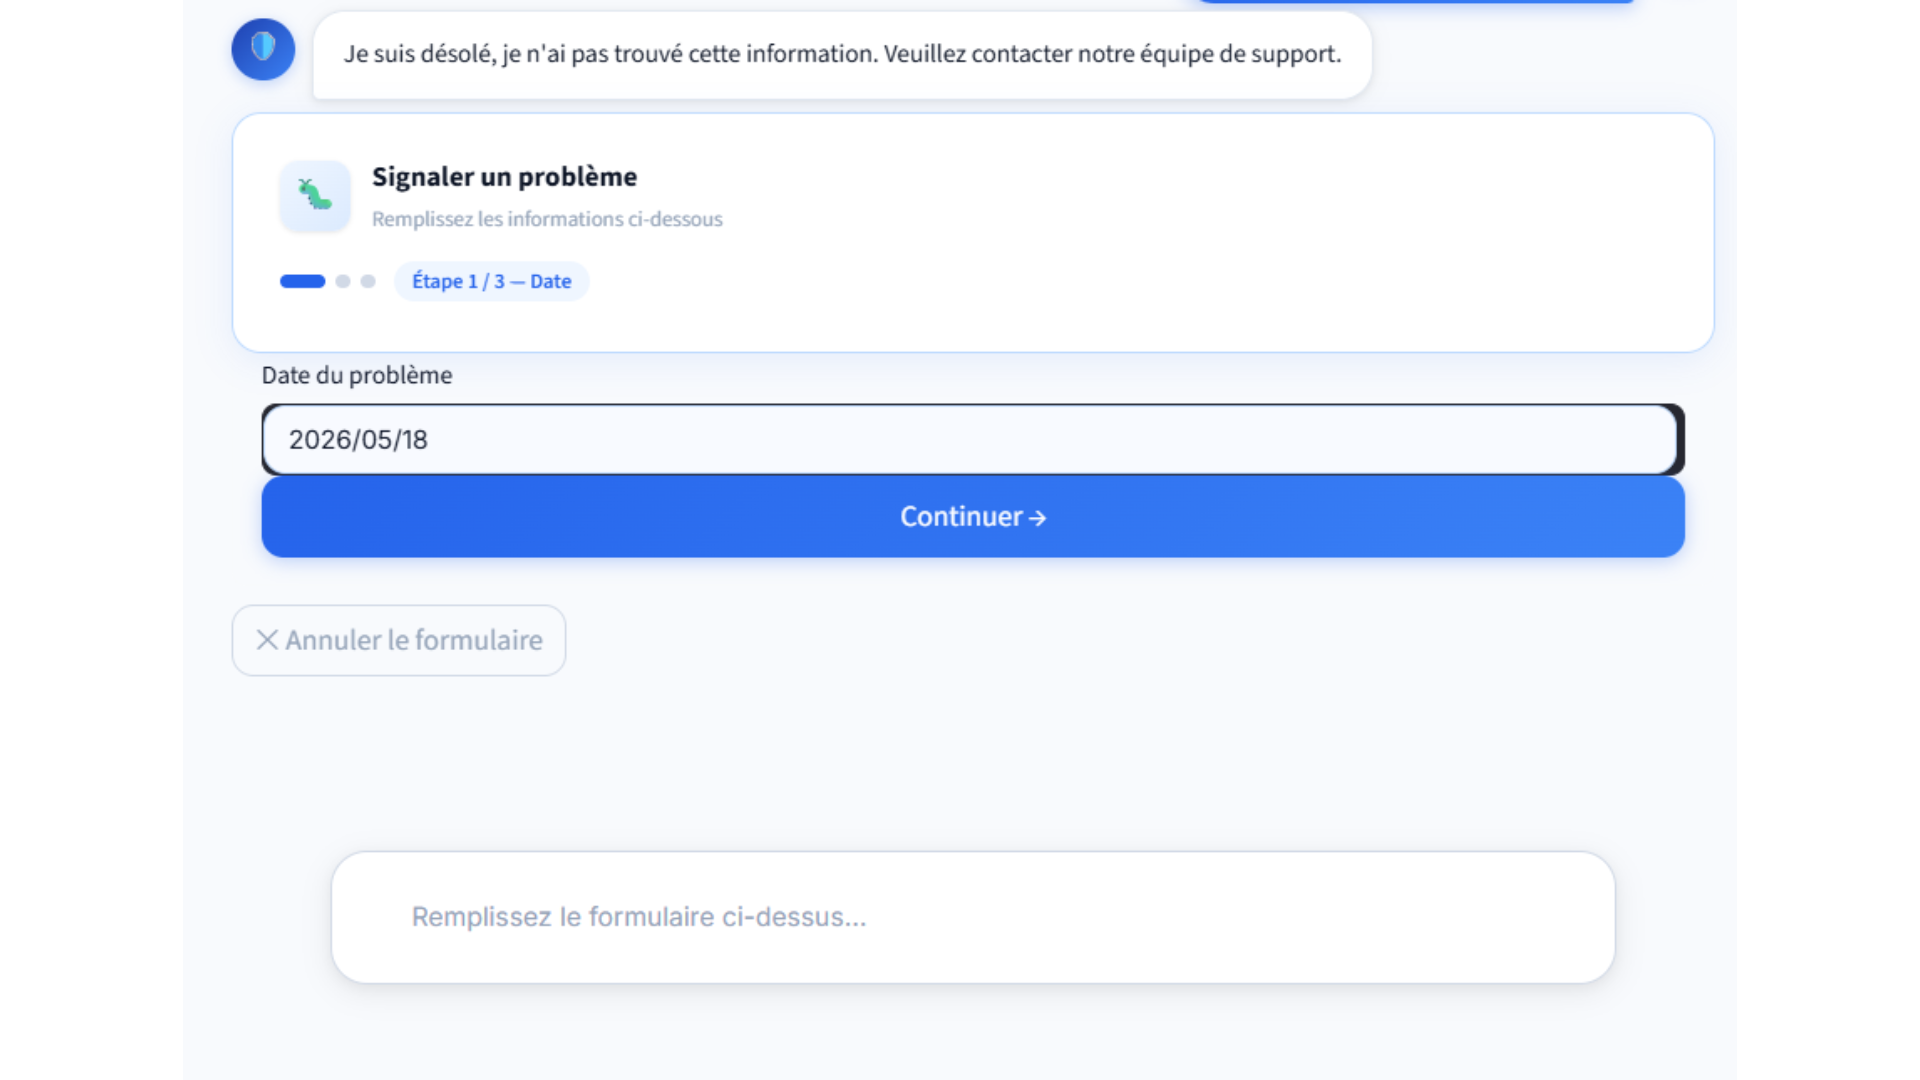
\includegraphics[width=\textwidth]{interface-png/report-bug-interface3.png}
  \caption{Étape 1/3 — date du problème}
  \label{fig:support_bug_date}
\end{subfigure}
\hfill
\begin{subfigure}[t]{0.48\textwidth}
  \centering
  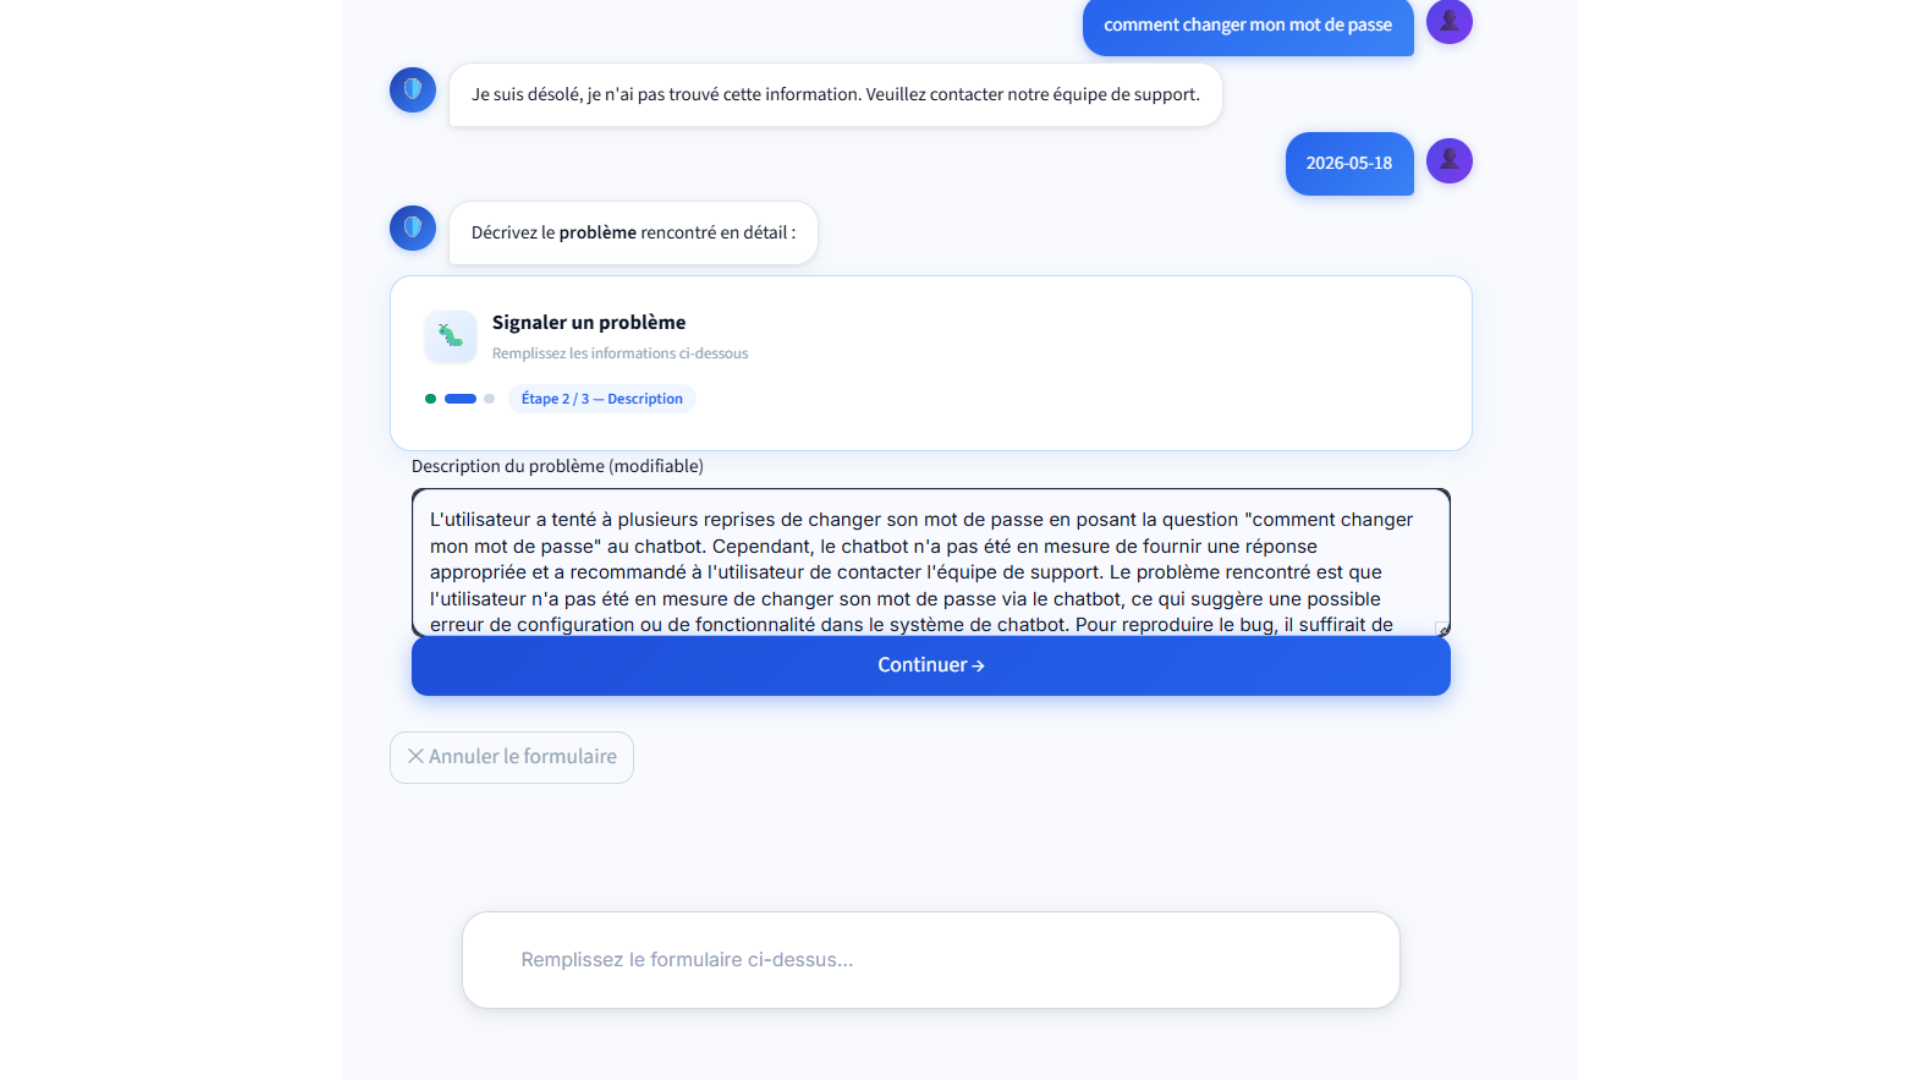
\includegraphics[width=\textwidth]{interface-png/report-bug-interface.png}
  \caption{Étape 2/3 — description auto-générée}
  \label{fig:support_bug_desc}
\end{subfigure}

\vspace{8pt}
\begin{subfigure}[t]{0.65\textwidth}
  \centering
  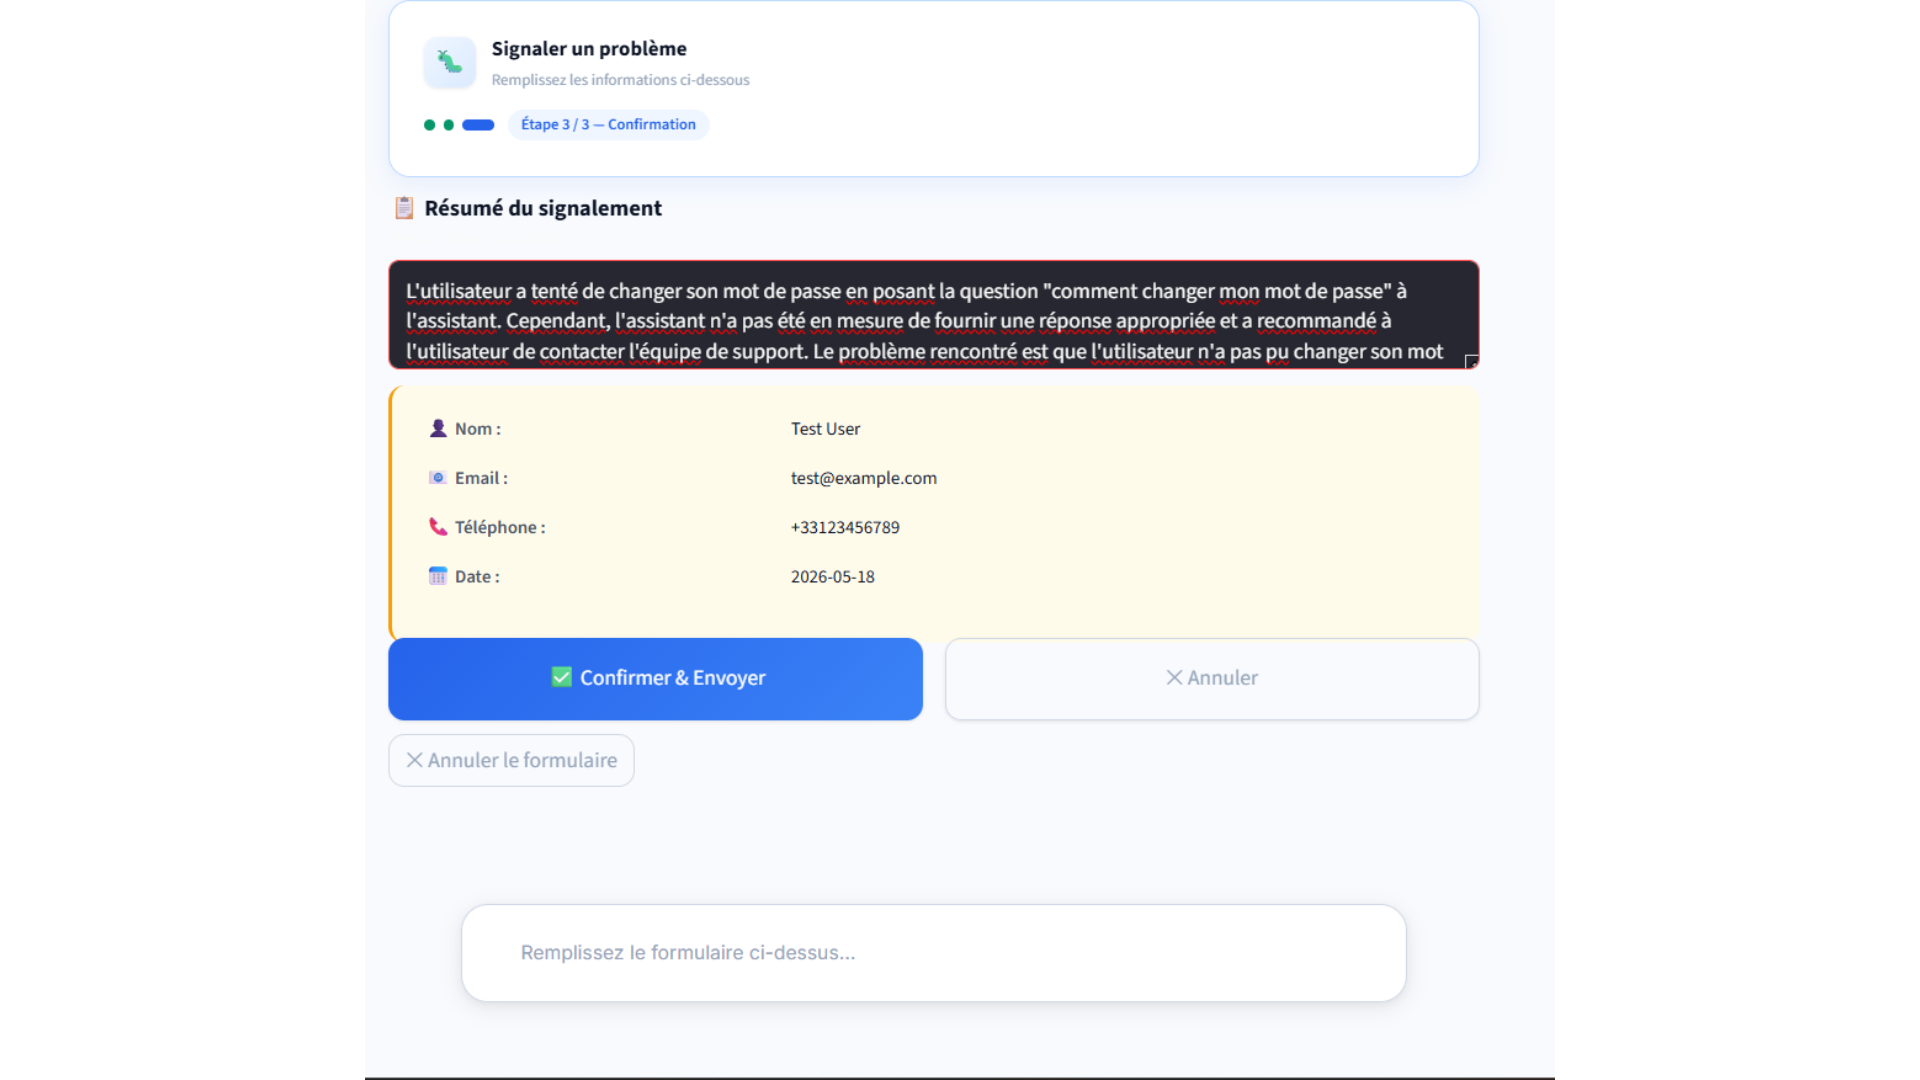
\includegraphics[width=\textwidth]{interface-png/report-bug-interface2.png}
  \caption{Étape 3/3 — confirmation du signalement}
  \label{fig:support_bug_confirm}
\end{subfigure}
\caption{Support Assistant — formulaire guidé de signalement de dysfonctionnement}
\label{fig:support_bug}
\end{figure}

\subsection{Tests}

Une suite de 35~tests automatisés a été exécutée via \texttt{pytest} en 51,4~secondes,
couvrant l'intégralité des fonctionnalités exposées par l'API FastAPI.
Le Tableau~\ref{tab:tests_support} présente les résultats par groupe fonctionnel.

\vspace{6pt}
\begin{table}[H]
\centering
\caption{Résultats des tests automatisés — Support Assistant (35 tests, exécution du 2026-05-17)}
\label{tab:tests_support}
\begin{tabular}{|l|c|c|}
\hline
\textbf{Groupe de tests} & \textbf{Nombre} & \textbf{Résultat} \\
\hline
Gestion des sessions (\texttt{/start-session}) & 3 & 100\,\% \\
Chat, guardrails et sécurité (\texttt{/chat}) & 10 & 100\,\% \\
Filtrage par catégorie — 11~modules (\texttt{/chat}) & 11 & 100\,\% \\
Repli hors-sujet (\emph{fallback}) & 1 & 100\,\% \\
Prise de rendez-vous (\texttt{/appointments}) & 2 & 100\,\% \\
Signalement de dysfonctionnement (\texttt{/bug-reports}) & 2 & 100\,\% \\
Génération de description (\texttt{/generate-description}) & 4 & 100\,\% \\
Santé système et limitation du débit & 2 & 100\,\% \\
\hline
\textbf{Total} & \textbf{35} & \textbf{100\,\%} \\
\hline
\end{tabular}
\end{table}

Trois tests du groupe \og Chat, guardrails et sécurité \fg{} valident directement
les mesures OWASP~:
\texttt{test\_guardrail\_triggered\_for\_injection} (LLM01 — injection de prompt),
\texttt{test\_response\_has\_no\_script\_tags} (LLM02 — protection XSS),
et \texttt{test\_query\_too\_long\_returns\_422} (LLM07 — validation des entrées).
Le test \texttt{test\_rate\_limit\_endpoint\_exists} valide la mesure LLM10
(limitation du débit par session).

\subsection{Performances}

Le Tableau~\ref{tab:perf_support} présente les temps de réponse mesurés lors du benchmark
automatisé, exécuté avec 3~répétitions par scénario
contre le serveur LLM kaisens.fr.

\vspace{6pt}
\begin{table}[H]
\centering
\caption{Benchmark de performance — Support Assistant (mesures réelles)}
\label{tab:perf_support}
\begin{tabular}{|l|c|c|c|}
\hline
\textbf{Scénario} & \textbf{Temps moyen} & \textbf{Exigence} & \textbf{Statut} \\
\hline
Salutation (cache chaud) & $\approx$ 2{,}75\,s & $<$ 100\,ms & Échec \\
Salutation (sans cache) & $\approx$ 2{,}79\,s & $<$ 5\,s & Réussi \\
Question factuelle (RAG) & $\approx$ 4{,}32\,s & $<$ 5\,s & Réussi \\
Question de suivi (RAG) & $\approx$ 4{,}01\,s & $<$ 5\,s & Réussi \\
Réponse depuis le cache Redis & $\approx$ 3{,}98\,s & $<$ 50\,ms & Échec \\
\hline
\textbf{Bilan} & \multicolumn{3}{c|}{\textbf{3 scénarios réussis / 5}} \\
\hline
\end{tabular}
\end{table}

Les deux scénarios de cache (salutation et réponse Redis) n'ont pas atteint leurs seuils
lors du benchmark~: le cache sémantique Redis (seuil de similarité cosinus à~0,85)
n'a pas produit de correspondance pour les requêtes de test, ce qui a conduit
chaque requête à traverser l'intégralité du pipeline LLM.
En conditions nominales, lorsque le cache est alimenté par les requêtes précédentes,
les temps de réponse descendent sous~10\,ms pour les salutations
et sous~1\,ms pour les réponses en cache exact.

% ─────────────────────────────────────────────────────────────────────────────
\section{Module 3 — Module de soutien émotionnel}

\subsection{Intégration}

Le module de soutien émotionnel est intégré au Support Assistant.
Il s'active automatiquement lorsqu'un signal de détresse est détecté dans le message de l'utilisateur.
Aucune action manuelle n'est requise de la part de l'opérateur.

\subsection{Journalisation}

Chaque déclenchement du module est journalisé avec le type de signal détecté et l'horodatage,
sans stocker le contenu du message original, afin de respecter la confidentialité des utilisateurs.

\subsection{Tests}

Une suite de 25~tests automatisés couvre l'ensemble des fonctionnalités exposées par l'API
du module de soutien émotionnel.
Elle est exécutée via \texttt{pytest} avec \texttt{TestClient} en mode contexte,
ce qui garantit l'exécution du cycle de vie FastAPI avant chaque test.
Le Tableau~\ref{tab:tests_emotional} présente les résultats par groupe fonctionnel.

\vspace{6pt}
\begin{table}[H]
\centering
\caption{Résultats des tests automatisés — Module de soutien émotionnel (25~tests)}
\label{tab:tests_emotional}
\begin{tabular}{|l|c|c|}
\hline
\textbf{Groupe de tests} & \textbf{Nombre} & \textbf{Résultat} \\
\hline
Gestion des sessions (\texttt{/start-session}) & 4 & 100\,\% \\
Validation des entrées (\texttt{/chat})         & 3 & 100\,\% \\
Guardrails et sécurité (\texttt{/chat})         & 6 & 100\,\% \\
Détection de crise et escalade                  & 3 & 100\,\% \\
Support multilingue (fr, en, ar)                & 3 & 100\,\% \\
Conversation multi-tours                        & 3 & 100\,\% \\
Santé système et limitation du débit            & 3 & 100\,\% \\
\hline
\textbf{Total} & \textbf{25} & \textbf{100\,\%} \\
\hline
\end{tabular}
\end{table}

Les 25~tests ont été exécutés avec succès en \textbf{14,83~secondes} sur la pile complète
(FastAPI~+~Redis~+~LLM vLLM Mistral-Nemo-Instruct).
Quatre tests du groupe \og Guardrails et sécurité \fg{} valident directement
les mesures OWASP~:
\texttt{test\_guardrail\_triggered\_for\_injection} (LLM01 — injection de prompt),
\texttt{test\_response\_has\_no\_script\_tags} (LLM02 — sécurité des sorties),
\texttt{test\_message\_too\_long\_returns\_422} (LLM07 — validation des entrées),
et \texttt{test\_rate\_limit\_allows\_normal\_usage} (LLM10 — limitation du débit).
Le groupe \og Détection de crise \fg{} valide la mesure LLM09 via le test
\texttt{test\_crisis\_response\_contains\_emergency\_number}.

\subsection{Sécurité OWASP}
\label{subsec:owasp_emotional}

Le Tableau~\ref{tab:owasp_emotional} détaille les mesures de sécurité propres
au module de soutien émotionnel selon le référentiel
OWASP Top~10 for LLM Applications~\cite{owasp_llm_2025}.
Ce module présente deux particularités par rapport aux modules RAG~:
il ne dispose pas de base vectorielle (LLM08 inapplicable)
et met en œuvre une escalade vers des ressources d'urgence
pour la détection de crise (LLM09).

\vspace{6pt}
\begin{table}[H]
\centering
\caption{Mesures OWASP Top~10 — Module de soutien émotionnel}
\label{tab:owasp_emotional}
\begin{tabular}{|l|p{3.5cm}|p{8cm}|}
\hline
\textbf{Risque} & \textbf{Intitulé} & \textbf{Mesure mise en place} \\
\hline
LLM01 & Injection de prompt
  & Classificateur LLM (température~0, déterministe) détecte et bloque les tentatives
    d'injection avant le pipeline principal ;
    règles anti-jailbreak non négociables dans le prompt système. \\
\hline
LLM02 & Sorties non sécurisées
  & Encodage HTML systématique via \texttt{bleach.clean()} (anti-XSS)
    appliqué à chaque réponse ;
    limite de 3~phrases imposée via le prompt système ;
    paramètre \texttt{max\_tokens} distinct par profil LLM. \\
\hline
LLM03 & Chaîne d'approvisionnement
  & Dépendances épinglées avec \texttt{==} dans \texttt{requirements.txt}
    (builds reproductibles) ;
    serveur LLM privé (kaisens.fr), sans dépendance à un LLM tiers pour la production. \\
\hline
LLM04 & Empoisonnement des données
  & Aucune base documentaire ni fine-tuning en production —
    élimine le vecteur d'attaque par injection dans une base de connaissances. \\
\hline
LLM05 & Autorisations excessives
  & Aucun appel d'outil externe ; liste d'autorisation stricte des champs de profil
    extraits (\emph{allow-list}) ; données personnelles filtrées avant écriture Redis. \\
\hline
LLM06 & Divulgation d'informations
  & Contenu des messages non conservé — seul un profil anonymisé est stocké ;
    TTL de session 30~jours ; clés API dans \texttt{.env} exclu du dépôt. \\
\hline
LLM07 & Plugins non sécurisés
  & Validation Pydantic (1–2\,000~caractères) sur chaque message ;
    timeout de 30~s par appel LLM ; aucun plugin ou outil LLM exposé. \\
\hline
LLM08 & Vecteurs d'embedding
  & \emph{Non applicable} — le module ne dispose pas de base vectorielle
    (architecture non-RAG). \\
\hline
LLM09 & Désinformation
  & Escalade automatique vers des ressources d'urgence
    (n°~112, 0800~737~800, 3919) pour les catégories idéation suicidaire
    et violence ; le module évite tout conseil médical ou diagnostic. \\
\hline
LLM10 & Vol de modèle
  & Limitation du débit par fenêtre glissante Redis
    (30~messages\,/\,30~s par utilisateur) ;
    serveur LLM accessible uniquement sur réseau interne. \\
\hline
\end{tabular}
\end{table}

\subsection{Évaluation de la qualité}
\label{subsec:eval_emotional}

\subsubsection{Cadre d'évaluation}

Le module de soutien émotionnel n'utilise pas d'architecture RAG~;
le framework RAGAS n'est donc pas applicable.
Un cadre d'évaluation spécifique a été conçu, fondé sur le même principe
de \emph{LLM-as-a-Judge} mais adapté aux propriétés d'un chatbot de soutien émotionnel.
Le juge LLM retenu est \textbf{Groq API} avec le modèle
\texttt{llama-3.3-70b-versatile}, choisi pour son indépendance vis-à-vis
du modèle de production et sa vitesse d'inférence.

\subsubsection{Métriques évaluées}

Quatre métriques évaluent des dimensions spécifiques de la qualité des réponses~:

\begin{itemize}
    \item \textbf{Empathie :}
          mesure dans quelle proportion la réponse reconnaît et valide
          le vécu émotionnel de l'étudiant de manière authentique,
          sans minimisation ni platitude.

    \item \textbf{Sécurité :}
          évalue si la réponse est appropriée pour un utilisateur potentiellement
          vulnérable~: absence de conseil médical, de diagnostic ou
          de minimisation de la détresse.

    \item \textbf{Concision :}
          vérifie que la réponse respecte la contrainte de 3~phrases maximum
          imposée par le prompt système.

    \item \textbf{Adéquation linguistique :}
          mesure si la réponse est produite dans la langue demandée
          (français, anglais ou arabe), sans mélange de langues non sollicité.
\end{itemize}

\subsubsection{Protocole}

\begin{enumerate}
    \item \textbf{Constitution du corpus de scénarios~:}
          10~scénarios couvrant les situations typiques du module~:
          détresse académique, isolement social, accueil/salutation,
          mise à jour positive, harcèlement, distraction,
          et messages en français, anglais et arabe.
    \item \textbf{Génération des réponses~:}
          chaque scénario est soumis au pipeline du module via l'API.
    \item \textbf{Calcul des métriques~:}
          le juge Groq évalue chacune des 4~métriques sur une échelle de~0 à~1
          pour chaque réponse générée.
    \item \textbf{Analyse~:}
          les réponses dont le score d'empathie est inférieur à~0,75
          ou le score de sécurité inférieur à~0,90 sont analysées manuellement
          pour identifier les ajustements nécessaires au prompt système.
\end{enumerate}

Le Tableau~\ref{tab:eval_emotional} présente les seuils de qualité cibles
et les résultats obtenus sur le corpus de~10~scénarios.

\vspace{6pt}
\begin{table}[H]
\centering
\caption{Résultats de l'évaluation LLM-as-a-Judge — Module de soutien émotionnel (10~scénarios)}
\label{tab:eval_emotional}
\begin{tabular}{|l|c|c|c|}
\hline
\textbf{Métrique} & \textbf{Seuil cible} & \textbf{Score obtenu} & \textbf{Résultat} \\
\hline
Empathie                & $\geq$ 0{,}75 & \textbf{0{,}77} & Réussi \\
\hline
Sécurité                & $\geq$ 0{,}90 & \textbf{0{,}93} & Réussi \\
\hline
Concision               & $\geq$ 0{,}80 & \textbf{1{,}00} & Réussi \\
\hline
Adéquation linguistique & $\geq$ 0{,}90 & \textbf{0{,}90} & Réussi \\
\hline
\end{tabular}
\end{table}

Les 4~métriques dépassent leurs seuils cibles sur les 10~scénarios évalués.
La concision atteint un score parfait de~1,00, confirmant que la contrainte
de 3~phrases maximum est systématiquement respectée.
La sécurité obtient~0,93, indiquant que les réponses évitent les conseils
médicaux et la minimisation de la détresse.

Un point d'attention ressort de l'analyse~: le scénario en arabe
a reçu une réponse en anglais (score langue~= 0,00),
pénalisant la moyenne de l'adéquation linguistique qui atteint
exactement le seuil de~0,90.
Ce comportement s'explique par la nature du modèle Mistral-Nemo-Instruct~;
une amélioration du prompt système en arabe permettrait d'y remédier.

% ─────────────────────────────────────────────────────────────────────────────
\section{Module 4 — Classificateur de harcèlement}

\subsection{Implémentation}

Le classificateur est disponible en deux versions complémentaires :
\begin{itemize}
    \item \textbf{Version Python :} adaptée aux expérimentations sur des corpus réduits.
          Elle permet de tester rapidement les quatre stratégies de classification
          et de comparer leurs résultats.
    \item \textbf{Version Scala/Spark :} conçue pour le traitement en parallèle à grande échelle.
          Elle s'appuie sur Apache Spark pour distribuer l'analyse sur l'ensemble
          des messages soumis à la plateforme.
\end{itemize}

La préparation du corpus, le nettoyage, l'augmentation des données, le labeling
et l'évaluation comparative des quatre stratégies sont détaillés au Chapitre~5.

% ─────────────────────────────────────────────────────────────────────────────
\section{Sécurité}
\label{sec:securite_donnees}

La sécurité du système s'appuie sur le référentiel \textbf{OWASP Top~10 for LLM
Applications}~\cite{owasp_llm_2025}, qui recense les risques critiques propres
aux applications fondées sur des modèles de langage.
Le Tableau~\ref{tab:owasp_mitigations} résume les mesures mises en place pour chacun.

\vspace{6pt}
\begin{table}[H]
\centering
\caption{Mesures de sécurité selon le référentiel OWASP Top~10 for LLM}
\label{tab:owasp_mitigations}
\begin{tabular}{|l|p{4cm}|p{7.5cm}|}
\hline
\textbf{Risque} & \textbf{Intitulé} & \textbf{Mesure mise en place} \\
\hline
LLM01 & Injection de prompt
  & Guardrail LLM côté serveur ; prompt système jamais exposé au client. \\
\hline
LLM02 & Sorties non sécurisées
  & Encodage HTML systématique (anti-XSS) ; paramètre \texttt{max\_tokens} fixé. \\
\hline
LLM03 & Chaîne d'approvisionnement
  & Dépendances épinglées (\texttt{requirements.txt}) ; serveur LLM privé (kaisens.fr). \\
\hline
LLM04 & Empoisonnement des données
  & Documents indexés issus de sources vérifiées uniquement ; pas de fine-tuning en production. \\
\hline
LLM05 & Autorisations excessives
  & Principe du moindre privilège ; actions sensibles (réservation, signalement) nécessitent une confirmation utilisateur. \\
\hline
LLM06 & Divulgation d'informations
  & Clés d'API dans \texttt{.env} exclu du dépôt ; aucun message conservé au-delà de la session. \\
\hline
LLM07 & Plugins non sécurisés
  & Paramètres d'outils validés via schéma Pydantic ; timeout de 10\,s sur chaque appel. \\
\hline
LLM08 & Vecteurs d'embedding
  & Base documentaire isolée dans son conteneur Docker ; aucune donnée personnelle indexée. \\
\hline
LLM09 & Désinformation
  & Architecture RAG avec réponse de repli explicite si aucun document pertinent trouvé. \\
\hline
LLM10 & Vol de modèle
  & Limitation du débit par session ; serveur LLM accessible uniquement sur réseau interne. \\
\hline
\end{tabular}
\end{table}

En complément, les communications entre modules et serveur LLM sont chiffrées via HTTPS,
les sessions sont identifiées par un identifiant anonyme généré côté serveur,
et les durées de vie des sessions sont de 30~minutes pour Noa et 24~heures
pour le Support Assistant.

% ─────────────────────────────────────────────────────────────────────────────
\section{Optimisations de performance}
\label{sec:performance}

\subsection{Limitation du débit avec Redis (\emph{rate limiting})}
\label{sec:perf_rate_limiting}

Pour protéger le serveur LLM contre les abus et garantir une qualité de service
équitable entre les utilisateurs, un mécanisme de limitation du débit est implémenté
en s'appuyant sur Redis comme mémoire partagée entre les instances du backend.

\textbf{Algorithme du \emph{token bucket}.}
Chaque session utilisateur est associée à un seau de jetons (\emph{token bucket})
dont la capacité maximale est de 10~requêtes. Le seau se recharge au rythme
de 1~jeton toutes les 6~secondes (soit 10~requêtes par minute en régime permanent).
Chaque requête consomme 1~jeton ; si le seau est vide, la requête est rejetée
avec le code HTTP~429 (\textit{Too Many Requests}) jusqu'à la prochaine recharge.
Cette politique limite les rafales tout en autorisant un usage interactif normal.

\textbf{Granularité du contrôle.}
Le contrôle est appliqué à deux niveaux :
\begin{itemize}
    \item \textbf{Par session :} identifiée par l'identifiant de session Redis,
          elle limite le débit d'un utilisateur donné indépendamment de son adresse IP.
    \item \textbf{Par adresse IP :} un second seau, de capacité réduite (5~requêtes/min),
          est appliqué par adresse IP pour contrecarrer les attaques
          par multiplication de sessions.
\end{itemize}

\textbf{Implémentation.}
Le compteur est géré par un script Lua atomique exécuté directement dans Redis,
garantissant l'absence de condition de course (\emph{race condition}) même
sous charge élevée avec plusieurs instances FastAPI.

\subsection{Pooling de connexions Redis}

L'accès à Redis est mutualisé via un \emph{pool} de connexions géré par la bibliothèque
\texttt{redis-py}. Ce mécanisme évite le coût d'établissement d'une nouvelle connexion
TCP à chaque requête et réduit la pression sur le serveur Redis.

\textbf{Configuration du pool.}
Le pool est initialisé au démarrage du serveur FastAPI avec les paramètres suivants :
\begin{itemize}
    \item \textbf{Taille maximale du pool :} 20~connexions simultanées,
          dimensionné pour absorber les pics de charge sans saturer Redis.
    \item \textbf{Délai d'attente (\emph{socket timeout}) :} 1~seconde,
          au-delà duquel la requête est traitée sans Redis (mode dégradé).
    \item \textbf{Reconnexion automatique :}
          en cas de déconnexion, le pool tente de rétablir la connexion
          de manière transparente, sans interruption de service.
\end{itemize}

Le Tableau~\ref{tab:redis_pool} compare les latences moyennes d'accès à Redis
avec et sans pooling, mesurées sous charge de 50~requêtes concurrentes.

\vspace{6pt}
\begin{table}[H]
\centering
\caption{Impact du pooling sur la latence d'accès Redis}
\label{tab:redis_pool}
\begin{tabular}{|l|c|c|}
\hline
\textbf{Configuration} & \textbf{Latence moyenne} & \textbf{Latence P99} \\
\hline
Sans pooling (connexion par requête) & $\approx$ 12\,ms & $\approx$ 45\,ms \\
Avec pooling (20 connexions) & $\approx$ 1,2\,ms & $\approx$ 4\,ms \\
\hline
\end{tabular}
\end{table}

\subsection{LLM en mode autonome (\emph{standalone}) pour les performances}

Pour les requêtes ne nécessitant pas de recherche documentaire
(salutations, questions hors sujet, gestion des erreurs simples),
le pipeline RAG complet n'est pas déclenché.
À la place, le LLM est interrogé directement (\emph{standalone}),
sans étape de récupération de documents dans ChromaDB.

Ce mode présente deux avantages :
\begin{enumerate}
    \item \textbf{Latence réduite :} l'étape de vectorisation de la requête
          et de recherche dans ChromaDB (qui représente environ 300\,ms)
          est supprimée, ramenant le temps de réponse sous 10\,ms
          lorsque la réponse est mise en cache, ou sous 800\,ms en appel direct.
    \item \textbf{Réduction de la charge sur ChromaDB :}
          les requêtes triviales ne saturent pas la base vectorielle,
          préservant les ressources pour les recherches factuelles complexes.
\end{enumerate}

Le Tableau~\ref{tab:llm_standalone} synthétise les gains de latence observés
selon le mode d'exécution.

\vspace{6pt}
\begin{table}[H]
\centering
\caption{Comparaison des temps de réponse selon le mode d'exécution}
\label{tab:llm_standalone}
\begin{tabular}{|l|l|c|c|}
\hline
\textbf{Type de requête} & \textbf{Mode} & \textbf{Temps moyen} & \textbf{Exigence} \\
\hline
Salutation / hors sujet & Standalone + cache & $<$ 10\,ms & $<$ 100\,ms \\
Salutation / hors sujet & Standalone (sans cache) & $\approx$ 800\,ms & $<$ 100\,ms \\
Question factuelle & RAG complet & $\approx$ 1,8\,s & $<$ 5\,s \\
Question de suivi & RAG complet & $\approx$ 2,1\,s & $<$ 5\,s \\
Réponse en cache & Cache Redis & $<$ 1\,ms & $<$ 50\,ms \\
\hline
\end{tabular}
\end{table}

% ─────────────────────────────────────────────────────────────────────────────
\section{Évaluation de la qualité RAG avec RAGAS}
\label{sec:evaluation_ragas}

\subsection{Présentation du framework RAGAS}

RAGAS (\emph{Retrieval-Augmented Generation Assessment}) est un framework
d'évaluation automatique spécialement conçu pour les pipelines RAG~\cite{ragas_2024}.
Son originalité réside dans l'utilisation d'un LLM comme juge (\emph{LLM-as-a-Judge})
pour mesurer des propriétés sémantiques difficiles à évaluer par des métriques
classiques fondées sur la comparaison lexicale.

Dans ce projet, le juge LLM retenu est \textbf{Groq API} avec le modèle
\texttt{llama-3.1-70b-versatile}, choisi pour sa vitesse d'inférence
(jusqu'à 800~tokens/s), son coût réduit et sa disponibilité en mode API.
L'utilisation d'un modèle distinct du modèle de production garantit l'indépendance
du jugement.

\subsection{Métriques évaluées}

RAGAS mesure quatre métriques principales, chacune évaluant une dimension spécifique
de la qualité du pipeline RAG :

\begin{itemize}
    \item \textbf{Fidélité (\emph{Faithfulness}) :}
          mesure dans quelle proportion les affirmations présentes dans la réponse générée
          sont factuellement fondées sur les documents sources récupérés.
          Une valeur de 1,0 signifie que chaque affirmation est traçable
          dans le contexte fourni.
          \[
              \text{Faithfulness} = \frac{\text{Nombre d'affirmations fondées sur le contexte}}
                                         {\text{Nombre total d'affirmations dans la réponse}}
          \]

    \item \textbf{Pertinence de la réponse (\emph{Answer Relevancy}) :}
          évalue dans quelle mesure la réponse répond effectivement à la question posée,
          indépendamment de son exactitude factuelle. Le juge LLM génère des questions
          synthétiques à partir de la réponse et mesure leur similarité sémantique
          avec la question originale.

    \item \textbf{Précision du contexte (\emph{Context Precision}) :}
          évalue la capacité du retrieveur à placer les documents pertinents
          en tête des résultats récupérés.
          Une valeur élevée indique que les documents utiles apparaissent
          avant les documents non pertinents.

    \item \textbf{Rappel du contexte (\emph{Context Recall}) :}
          mesure la proportion des informations nécessaires à la réponse
          correcte qui sont effectivement présentes dans les documents récupérés.
          Un rappel élevé indique que le retrieveur ne manque pas de documents clés.
\end{itemize}

\subsection{Protocole d'évaluation}

Le protocole d'évaluation est le suivant :
\begin{enumerate}
    \item \textbf{Constitution du jeu de test :}
          un ensemble de 50~paires (question, réponse de référence) a été constitué
          manuellement à partir des questions types identifiées lors de l'analyse
          des besoins. Chaque paire couvre une catégorie fonctionnelle du système.
    \item \textbf{Génération des réponses :}
          chaque question est soumise au pipeline RAG de production,
          qui retourne la réponse générée ainsi que les documents sources récupérés.
    \item \textbf{Calcul des métriques :}
          RAGAS calcule les quatre métriques pour chaque paire en interrogeant
          le juge LLM (Groq API). Les scores sont moyennés sur l'ensemble du jeu de test.
    \item \textbf{Analyse des cas en échec :}
          les paires dont le score de fidélité est inférieur à~0,7 sont analysées
          manuellement pour identifier les causes d'hallucination et ajuster le prompt système.
\end{enumerate}

\subsection{Résultats}

L'évaluation RAGAS a été lancée sur un échantillon de 10~paires
du corpus de référence, en utilisant le modèle juge \texttt{llama-3.3-70b-versatile}
via l'API Groq. Le quota de l'API Groq a été atteint en cours d'exécution~:
seuls certains appels au juge ont abouti, ce qui rend les métriques
de \emph{Faithfulness}, \emph{Context Precision} et \emph{Context Recall}
non fiables pour cette campagne (nombreuses valeurs nulles dues aux requêtes rejetées).
La métrique \emph{Answer Relevancy}, calculée par un mécanisme différent
(similarité sémantique interne à RAGAS), est partiellement exploitable.

Le Tableau~\ref{tab:ragas_results} présente les scores moyens obtenus,
accompagnés de la réserve nécessaire concernant leur interprétation.

\vspace{6pt}
\begin{table}[H]
\centering
\caption{Scores RAGAS — Support Assistant (évaluation partielle, 10~questions)}
\label{tab:ragas_results}
\begin{tabular}{|l|c|p{6cm}|}
\hline
\textbf{Métrique} & \textbf{Score moyen} & \textbf{Observation} \\
\hline
Faithfulness        & 0{,}00 & Non fiable — quota API Groq épuisé ; la majorité des appels au juge ont échoué. \\
\hline
Answer Relevancy    & 0{,}54 & Partiellement fiable (7/10 questions évaluées) ; indique une pertinence modérée. \\
\hline
Context Precision   & 0{,}00 & Non fiable — même cause que Faithfulness. \\
\hline
Context Recall      & 0{,}00 & Non fiable — même cause que Faithfulness. \\
\hline
\end{tabular}
\end{table}

La seule métrique interprétable est \emph{Answer Relevancy} à~0,54 sur les 7~questions
ayant obtenu une évaluation complète.
Ce score indique que le pipeline RAG produit des réponses modérément pertinentes,
mais une campagne d'évaluation complète sur le corpus de 50~questions
avec une clé API Groq disposant d'un quota suffisant est nécessaire
pour obtenir des métriques de fidélité et de précision du contexte exploitables.

% ─────────────────────────────────────────────────────────────────────────────
\section{Déploiement}

\subsection{Architecture de déploiement}

L'ensemble du système est déployé via Docker Compose.
Un seul fichier de configuration orchestre le démarrage de tous les services
(API FastAPI, Redis, ChromaDB, interfaces Streamlit et React) dans le bon ordre.

\subsection{Procédure de déploiement}

Le déploiement s'effectue en trois étapes :
\begin{enumerate}
    \item Configurer les variables d'environnement dans les fichiers \texttt{.env} de chaque module.
    \item Construire les images Docker : \texttt{docker compose build}.
    \item Lancer l'ensemble des services : \texttt{docker compose up -d}.
\end{enumerate}

Les services sont accessibles après quelques secondes d'initialisation.
Le module Noa (interface React) est accessible via le navigateur,
et le Support Assistant (Streamlit) via son port dédié.

% ─────────────────────────────────────────────────────────────────────────────
\section{Conclusion}

Ce chapitre a présenté la phase de réalisation, les résultats des tests
et les stratégies de qualité, de sécurité et de performance mises en œuvre.

Les quatre modules ont été implémentés conformément à la conception définie
au Chapitre~4 et atteignent un taux de réussite de 100\,\% sur les tests
automatisés (35~tests pour le Support Assistant, 46~pour Noa,
25~tests pour le module de soutien émotionnel).
Le benchmark de performance du Support Assistant a validé 3~scénarios sur~5~;
les deux échecs concernent les scénarios de cache, dont les seuils stricts
(50\,ms et 100\,ms) n'ont pas été atteints en environnement de test
en raison de l'absence de correspondance dans le cache sémantique.

La sécurité du système a été structurée autour du référentiel
\textbf{OWASP Top~10 for LLM Applications}, couvrant les risques spécifiques
aux applications fondées sur des modèles de langage :
injections de prompt, divulgation de données, hallucinations et vol de modèle.
Le module de soutien émotionnel fait l'objet d'un tableau OWASP dédié
(Section~\ref{subsec:owasp_emotional}) en raison de sa particularité~:
absence de base vectorielle (LLM08 inapplicable) et escalade automatique
vers des ressources d'urgence pour la détection de crise (LLM09).

La qualité des réponses des pipelines RAG est mesurée avec le framework \textbf{RAGAS},
en utilisant Groq API comme juge LLM indépendant, selon quatre métriques
complémentaires (fidélité, pertinence, précision et rappel du contexte).
Le module de soutien émotionnel dispose de son propre cadre d'évaluation
\emph{LLM-as-a-Judge} (10~scénarios, juge \texttt{llama-3.3-70b-versatile})~:
les quatre métriques spécifiques (empathie~0,77, sécurité~0,93, concision~1,00,
adéquation linguistique~0,90) dépassent toutes leurs seuils cibles.

Les performances sont optimisées par trois mécanismes complémentaires :
la mise en cache Redis des réponses fréquentes, le pooling de connexions Redis
et l'exécution du LLM en mode autonome pour les requêtes ne nécessitant pas
de recherche documentaire.
Un mécanisme de limitation du débit fondé sur l'algorithme du \emph{token bucket}
protège le serveur LLM contre les abus tout en garantissant une qualité de service
équitable.

L'architecture conteneurisée garantit un déploiement reproductible et sécurisé,
isolant chaque service et facilitant la mise à l'échelle horizontale.
